\section{Arrays}

Adding support for arrays in \texttt{PArL} has driven a number
of changes across whole of the compiler. Some of these changes
will be explained in the following sections whilst otherwise
where already described in earlier section due to the
fundamental changes they caused.

\subsection{Changes in Lexical Analysis}

\begin{lstlisting}[caption={Changes in the
\texttt{LexerDirector} for supporting left (`\texttt{[}') and
right (`\texttt{]}') brackets (lexer/LexerDirector.cpp)}]
...

.addCategory(
    LEFT_BRACKET,
    [](char c) -> bool {
        return c == '[';
    }
)
.addCategory(
    RIGHT_BRACKET,
    [](char c) -> bool {
        return c == ']';
    }
)

...

.addTransition(0, LEFT_BRACKET, 20)
.addTransition(0, RIGHT_BRACKET, 21)

...

.setStateAsFinal(20, Token::Type::LEFT_BRACK)
.setStateAsFinal(21, Token::Type::RIGHT_BRACK)

...
\end{lstlisting}


Within lexical analysis a very lax approach to arrays was
adopted. That is there is no enforcement of the more complicated
$\langle$Identifier$\rangle$ syntax proposed in the original
EBNF of the language. The only additions have been support for
consuming left (`\texttt{[}') and right (`\texttt{]}') brackets.

\subsection{Changes in Parsing}

As described in \ref{sss:secarrays}, the grammar of the language
was significantly reordered to improve the upgrade-ability of
the language down the line. Additionally, the majority of the
changes to the parser where also discussed in
\ref{sss:secarrays}.

\begin{todo}
The addition of de-sugaring, type inference and more types is
facilitated by the changes proposed in the EBNF. These additions
would allow for more complicated language mechanisms and hence
an improved developer experience down the line.
\end{todo}

\subsection{Changes in Semantic Analysis}

Again due to the changes in the way types are managed, (again
see \ref{sss:primitive}), this leads to a number of notable
changes in particular: extra validation is necessary,
restriction on type casting, figuring out the type of array
access and finally, generating the type for array literals.

\begin{lstlisting}[caption={A part of the \texttt{visit(Binary
*)} method in the \texttt{AnalysisVisitor} class
(analysis/AnalysisVisitor.cpp)}]
...
case core::Operation::ADD:
case core::Operation::SUB:
    if (leftType.is<core::Array>()) {
        error(
            expr->position,
            "operator {} is not defined on array "
            "types",
            core::operationToString(expr->op)
        );
    }

    if (leftType != rightType) {
        error(
            expr->position,
            "operator {} expects both operands to "
            "be of same type",
            core::operationToString(expr->op)
        );
    }

    mReturn = leftType;
    break;
...
\end{lstlisting}

Of course validation is necessary to ensure that arrays do no
interact with each other, for example \texttt{[1,2,3] + [1,2,3]}
is not semantically, correct in \texttt{PArL}.

\begin{lstlisting}[caption={The \texttt{isViableCast()} method
in the \texttt{AnalysisVisitor} class
(analysis/AnalysisVisitor.cpp)}]
void AnalysisVisitor::isViableCast(
    core::Primitive &from,
    core::Primitive &to

) {
    const core::Primitive *lPtr = &from;
    const core::Primitive *rPtr = &to;

    while (lPtr != nullptr && rPtr != nullptr) {
        if (lPtr->is<core::Base>() &&
            rPtr->is<core::Array>()) {
            error(
                mPosition,
                "primitive cannot be cast to an array"
            );
        }

        if (lPtr->is<core::Array>() &&
            rPtr->is<core::Base>()) {
            error(
                mPosition,
                "array cannot be cast to a primitive"
            );
        }

        if (lPtr->is<core::Array>() &&
            rPtr->is<core::Array>()) {
            size_t lSize = lPtr->as<core::Array>().size;
            size_t rSize = rPtr->as<core::Array>().size;

            lPtr = lPtr->as<core::Array>().type.get();
            rPtr = rPtr->as<core::Array>().type.get();

            if (lSize != rSize) {
                error(
                    mPosition,
                    "array of size {} cannot be cast to an "
                    "array of size {}",
                    lSize,
                    rSize
                );
            }

            continue;
        }

        return;
    }

    core::abort("unreachable");
}
\end{lstlisting}

Necessary checks to ensure that casting is viable, need to be
considered. This approach was taken over allowing all forms of
casting because casting from one type to another where the sizes
of the types are different would result in substantial
complexity later on in code generation.

Consider the following example:

\begin{center}
\begin{minipage}[l]{0.54\linewidth}
\begin{lstlisting}[morekeywords={color}]
let x: int[5] = [1,2,3,4,5];
let y: int = (x as color[10])[6];
\end{lstlisting}
\end{minipage}
\end{center}

Not only is there ambiguity as to what the upper elements of the
type cast should be but the additional elements are necessary to
ensure no out of of bounds accesses during VM execution.

Finally, the process of computing the type of an array access
and an array literal is quite easy, see
analysis/AnalysisVisitor.cpp lines 252 and 170 respectively.

\subsection{Changes in Code Generation}

One of the more important changes for code generation is the
calculation of frame sizes. This has already been described in
detail even in the context of arrays in the note in subsection
\ref{sss:framesizecalc}. Of course where appropriate
\texttt{sta}, \texttt{pusha}, \texttt{printa} and \texttt{push
+[i:l]} which are for storing arrays, pushing arrays onto the
operand stack, printing arrays and pushing an single element of
the array onto the operand stack respectively, are being used
accordingly. See ir\_gen/GenVisitor.cpp, lines 456, 111, 478 and
166, for examples of each.

A decision to opt out of using \texttt{reta} was made due to the
inconsistent behaviour of arrays in the VM. Instead a hack for
reversing the order manually was devised.

\begin{lstlisting}[caption={A part of the \texttt{visit(Variable
*)} method in the \texttt{GenVisitor} class, specifically the
hack mentioned above (ir\_gen/GenVisitor.cpp)},label=lst:hack]
...
if (symbol.type.is<core::Array>()) {
    size_t arraySize =
        symbol.type.as<core::Array>().size;
    emit_line("push {}", arraySize);
    emit_line("pusha [{}:{}]", symbol.idx, level);
    emit_line("push {} // START HACK", arraySize);
    emit_line("oframe");
    emit_line("push {}", arraySize);
    emit_line("push 0");
    emit_line("push 0");
    emit_line("sta");
    emit_line("push {}", arraySize);
    emit_line("pusha [0:0]");
    emit_line("cframe // END HACK");

    return;
}
...
\end{lstlisting}

The problem of arrays is the following:

Consider the following code: \texttt{\_\_print [1,2,3];}

\begin{minipage}[l]{0.2\linewidth}
\begin{lstlisting}[morekeywords={push, printa, oframe, cframe,
halt}]
  .main
  push 0
  oframe
  push 3
  push 2
  push 1
  push 3
  printa
  cframe
  halt
\end{lstlisting}
\end{minipage}
\hfill\begin{minipage}[t][10em][t]{0.7\linewidth}
It generates the code on the left and what is important to
notice is the last element in the array is the first to be
pushed onto the operand stack ensuring that printing is correct.
\end{minipage}

However, now consider the following piece of code: \texttt{let
x: int[3] = [1,2,3]; \_\_print x;}

\begin{minipage}[l]{0.2\linewidth}
\begin{lstlisting}[morekeywords={sta, push, pusha, printa, oframe,
cframe, halt}]
  .main
  push 3
  oframe
  push 3
  push 2
  push 1
  push 3
  push 0
  push 0
  sta
  push 3
  pusha [0:0]
  push 3
  printa
  cframe
  halt
\end{lstlisting}
\end{minipage}
\hfill\begin{minipage}[t][10em][t]{0.7\linewidth}
The nïve implementation generates the code on
the left. Running this on the VM one would
expect the exact same output as the first.
However, this is not the case the order of the
elements is reversed.
\end{minipage}

\begin{figure}[H]
    \centering
    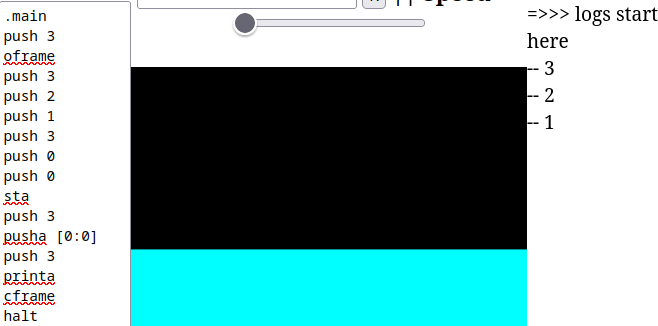
\includegraphics[width=\linewidth]{naivepusha.png}
    \caption{The result of running the code generated
    \texttt{let x: int[3] = [1,2,3]; \_\_print x;} in the VM}
\end{figure}

This happens because reading from a frame using \texttt{pusha}
actually reverse the order of the elements on the operand stack.
To circumvent this issue a second temporary frame is created
where the elements are stored in the frame and read again
reversing the order one-more time into the correct order (see
\listref{hack}).

Due to this change hack which works in all situations
\texttt{reta} is not being used as the would flip the order
again.
